%http://www.imn.htwk-leipzig.de/~schwarz/lehre/ss17/dbv/projekte-ss17.pdf

\chapter{Programmfunktion}\label{sec:Einleitung}
Das vorliegende ImageJ-Plugin Flowig dient zur Erkennung der Bewegung eines markierten Objektes in Bildfolgen. Es wird für jedes Bild die Bewegung des Objekts im Vergleich zum vorherigen Bild erkannt. Zudem wird der optische Fluss berechnet.

\textbf{Eingabe: } Ein Ordner, in dem sich eine Bildfolge befindet. Ist ein Objekt in einem Bild vorhanden, muss dieses durch Bounding-Boxen markiert sein.


\textbf{Ausgabe: } Bewegungsrichtung und Geschwindigkeit des Objekts in jedem Bild


\textbf{Anzeige: } Bewegungsrichtungen auf jedem Bild als Overlay und Darstellung des optischen Flusses

\section{Installation}
%TODO flowig.java muss in plugins/flowig liegen
Die Datei \code{Flowig\_.java} muss in einem eigenen Unterordner \code{flowig} in ImageJ's Plugin Ordner liegen.

Flowig nutzt die Bibliothek JavaCV~\footnote{\url{https://github.com/bytedeco/javacv}}. Damit auf die Bibliothek zugegriffen werden kann, müssen zuerst die Dateien \code{javacpp.jar, javacv.jar, opencv.jar} und \code{opencv-linux-x86\_64.jar} in den Ordner \code{ImageJ/plugins/jars} kopiert werden.

Des Weiteren muss die Version des genutzten Plugin-Compilers auf $1.8$ eingestellt sein. 
Die aktuelle Version lässt sich in ImageJ über folgendes Menü einsehen:\\
\mbox{\textbf{Edit}~$\rightarrow$~\textbf{Options}~$\rightarrow$~\textbf{Compiler\dots}} 

\section{Nutzung}

Nachdem das Plugin gestartet wurde, muss ein Ordner gewählt werden, der eine Bildfolge enthält.

Nach Anwenden des Plugins auf die geöffnete Bildfolge, wird in der Konsole die Bewegungsrichtung, sowie die Geschwindigkeit des Objekts in jedem Bild ausgegeben.

Für jedes Bild wird zudem ein Overlay erstellt, das die Änderung der Position im Vergleich zum vorherigen Bild in Form von Pfeilen darstellt. Abbildung \ref{img:bsp2} zeigt ein beispielhaftes Overlay. Dort wird die Bewegung des Objekts von Abbildung \ref{img:bsp1} zu Abbildung \ref{img:bsp2} dargestellt.
 
Der beispielhafte optische Fluss zu Bild \ref{img:bsp2} wird in Abbildung \ref{img:bsp3} dargestellt. Jeder Pixel bekommt einen Farbwert zugewiesen. Das Zuweisen geschieht über die Auswahl einer Farbe in einem Farbrad. Die Richtung des Vektors des Pixels im optischen Fluss bestimmt den Farbton, der Betrag des Vektors bestimmt die Sättigung. Es wird zudem eine Legende angezeigt, ein beispielhaftes Farbrad wird in Bild \ref{img:bsp4} gezeigt.

\begin{figure}[p]
	%\hskip-1.0cm
	\centering
	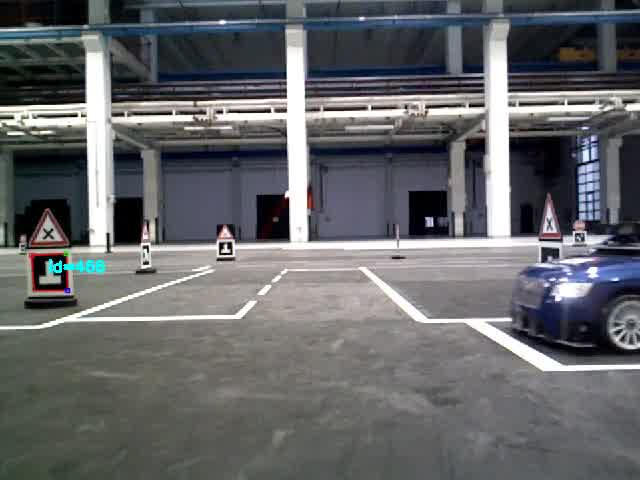
\includegraphics[scale=0.5]{./Abbildungen/bsp1.jpg}
	\caption{Ein Eingabebild ohne Overlay}
	\label{img:bsp1}
\end{figure}

\begin{figure}[p]
	%\hskip-1.0cm
	\centering
	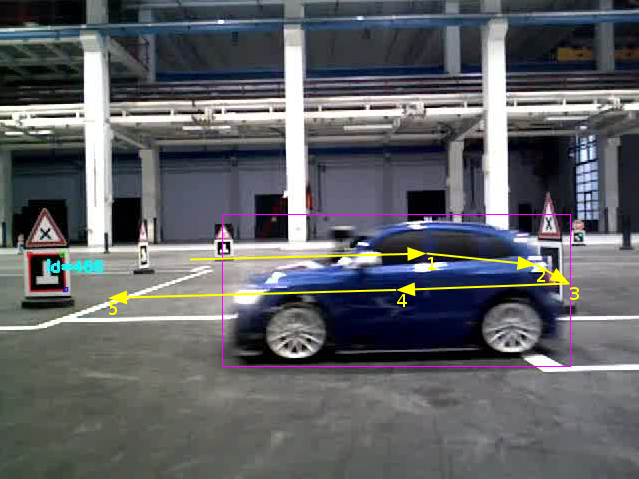
\includegraphics[scale=0.5]{./Abbildungen/4.png}
	\caption{Bewegung zu Beispiel 1}
	\label{img:bsp2}
\end{figure}

\begin{figure}[p]
	%\hskip-1.0cm
	\centering
	
\includegraphics[scale=0.5]{./Abbildungen/5.png}
	\caption{Optischer Fluss zu \ref{img:bsp2}}
	\label{img:bsp3}
\end{figure}

\begin{figure}[p]
	%\hskip-1.0cm
	\centering
	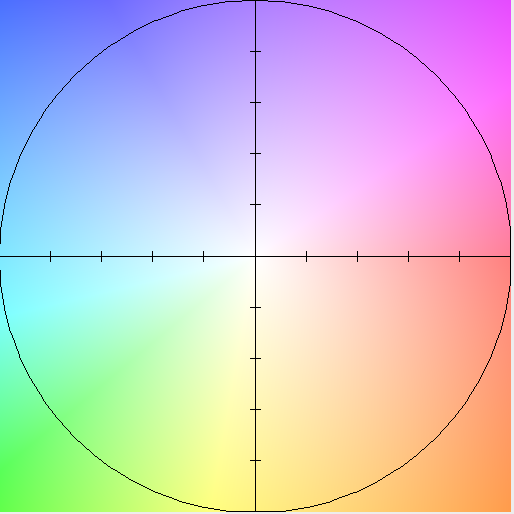
\includegraphics[scale=0.5]{./Abbildungen/6.png}
	\caption{Beispielhaftes Farbrad}
	\label{img:bsp4}
\end{figure}

\section{Aufruf über Kommandozeile}

Damit das Plugin über die Kommandozeile aufgerufen werden kann, muss man es mindestens einmal über \textbf{Compile and Run\dots} ausführen. Daraufhin kann man es über folgenden Befehl aufrufen:

\code{ImageJ -macro /flowig/macro/runplug.ijm Flowig\#parameter=<wert>,\dots}


Mögliche Parameter:

\code{path=dir} ist der Ordner, der die Bildfolge enthält.
 \\

\code{flow=flowType} stellt den zu nutzenden Algorithmus zur Berechnung des optischen Flusses dar, es können folgenden Typen angegeben werden:

\begin{itemize}
\item SparseToDense
\item FarneBack
\item DeepFlow
\item DIS
\item DualTVL1
\end{itemize}

Standardwert: DIS 

\code{showx=true|false} und \code{showy=true|false} schalten die Darstellung der $x$ beziehungsweise $y$ Komponenten des optischen Flusses ein und aus, Standardwerte: true

\code{boundscolor} ist die Farbe der Bounding-Boxen im Format: <r>+<g>+<b>, Standardwert: 255+255+0

\code{maxmotion} der Maximalwert der Farbintensitätsskalierung, Standardwert: 100

\code{scalesize} gibt an, wie oft das Bild herunterskaliert wird für die Flussberechnung, Standardwert: 0

\code{scalecolor} gibt den Sättigungsmultiplikator an, Standardwert: 1


Ist während der Ausführung keine grafische Oberfläche erwünscht, so ist \code{-macro} durch \code{-batch} zu ersetzen.